\documentclass{article}
\usepackage[utf8]{inputenc}
\usepackage{graphicx}
\usepackage[margin=1in]{geometry}
\usepackage{subfig}
\usepackage{enumitem}
\usepackage{hyperref}

\graphicspath{{./img/}{./images/}}

\title{Report}
\author{Yuji Akimoto, Kenta Takatsu, Chetan Velivela}
\date{May 2018}

\begin{document}

\begin{titlepage}
    \begin{center}
        \vspace*{1cm}
        
        \textbf{
            \LARGE{QuACC: \\ Question Answering for Cornell Courses} \\
            \vspace{0.5cm}
            \large{Spring 2018 Report}
        }
        
        \vspace{1.5cm}
        Yuji Akimoto \\
        Kenta Takatsu \\
        Chetan Velivela
        
        \vspace{4cm}
        \begin{figure}[h]
            
\includegraphics[width=8cm]{nlp_research.png}
            \centering
        \end{figure}
        
        \vfill
        Cornell Data Science \\
        \today
        
    \end{center}
\end{titlepage}

%% INTRODUCTION
\section{Introduction}
As one of the many abilities required in order for a computer to achieve artificial general intelligence, the capacity for an algorithm to extract knowledge from a passage of text has attracted increasing attention in recent years. Referred to interchangeably as reading comprehension (RC), machine comprehension (MC), and question answering (QA), this task involves answering questions about any given passage of text, much like one may find on the SAT. \\

Despite recent advances in natural language processing, this task has proven difficult for a number of reasons. The first is simply the intrinsic difficulty of the task itself: answering what may appear to be simple questions often require a large amount of general knowledge and hierarchical reasoning that we often dismiss as ``common sense''. Take for example the statement ``San Jose Sharks pursuing free agent John Tavares''. Without the background knowledge that the San Jose Sharks are a professional sports team, or that free agents refer to players without a contract, it is easy to misunderstand that some sort of spy is literally being chased by sharks. The second is the lack, until recently, of an industry-standard task analogous to the ImageNet challenge that spurred many advances in computer vision. To this end, the release of the Stanford Question Answering Dataset (SQuAD) \cite{SQuAD}, represents a significant advancement in the field. This dataset consists of over 100,000 questions on Wikipedia articles, where the answer to every question is a subsection of a relevant article. Specifically, each sample consists of four identifiers: a paragraph containing relevant information, a question, and pointers (in the paragraph) to the beginning and end of the answer; a sample is shown in Figure~\ref{fig:squadExample}.

\begin{figure}[h]
	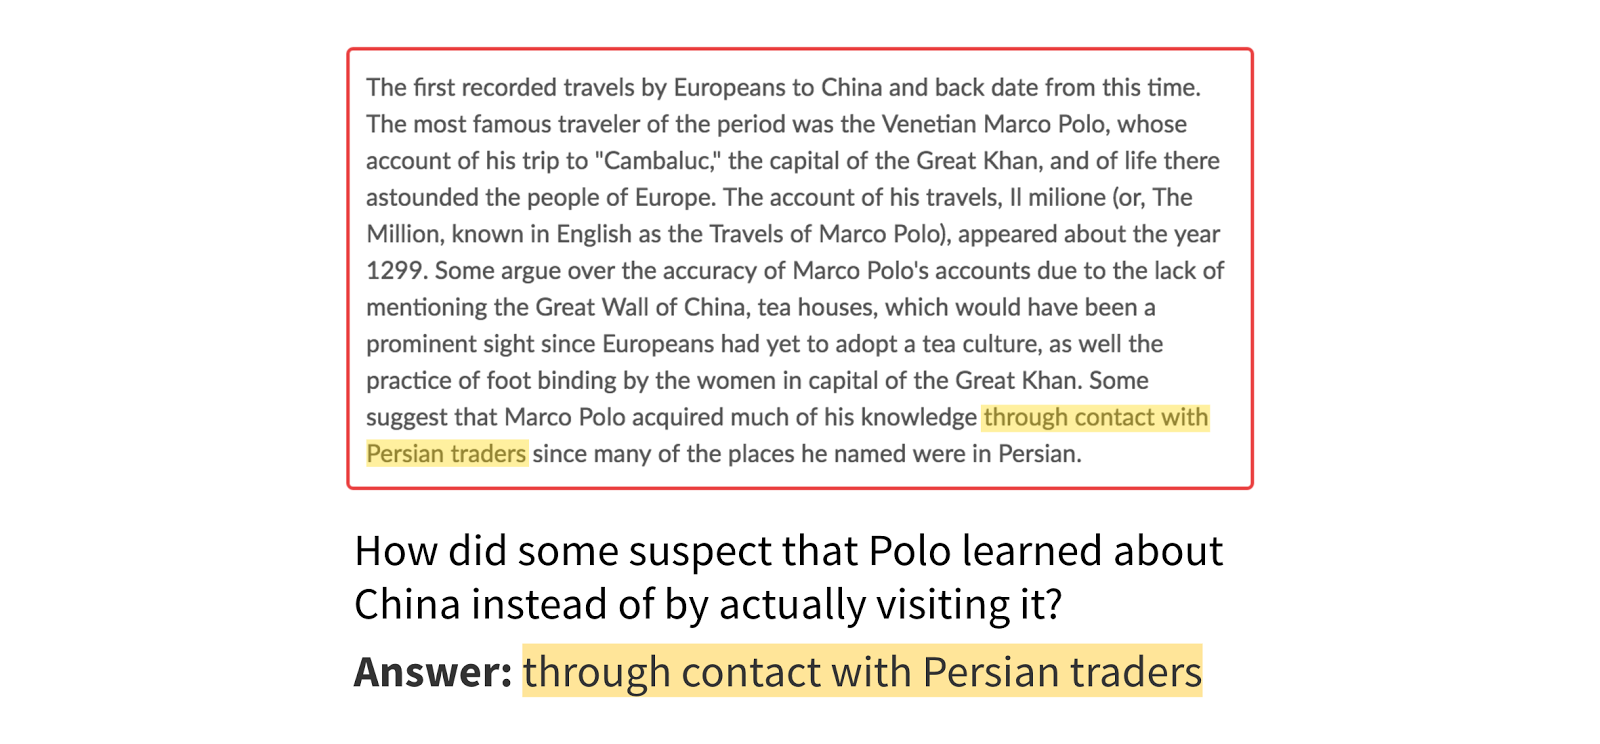
\includegraphics[width=0.8\textwidth]{squad_example.png}
	\centering
	\caption{A sample from the SQuAD dataset}
	\label{fig:squadExample}
\end{figure}

Our goal for the semester has been to develop an algorithm to perform well on the SQuAD dataset, while gaining understanding about the algorithms that others have designed for this task and exploring possible adapations. In the long term, we hope to implement an end-to-end system that is capable of answering questions about courses at Cornell (hence the title) through the online Q\&A service Piazza. 

%% BACKGROUND
\section{Background} \label{background}
Almost all of the work in this field relies on recurrent neural networks (approaches using convolutional nets have focused on computation considerations at the cost of increasing the number of parameters \cite{CNN_QA}). Specifically, most related works use attention-based recurrent neural networks, which we outline below. We also outline other major steps in designing an end-to-end recurrent neural network for natural language processing tasks.

\subsection{Pre-trained Embeddings}
Although words are theoretically categorical in that there exists a finite number of words in the English language, it is not efficient to use one-hot encodings for two main reasons: the large number of proper nouns found in Wikipedia articles makes the set of unique tokens very large, and attempts to learn the semantic similarity of words through the contexts in which they appear have proven successful. To address the second point, we use pre-trained GloVe \cite{GloVe} vectors to encode the meaning of passages of text. Similarly to word2vec \cite{word2vec}, GloVe produces vector space embeddings of words where geometric relationships are reflective of semantic relationships, which as shown in Figure~\ref{fig:gloveExample}, extend to proper nouns. Several versions of GloVe exist, but we use the 300-dimensional embeddings with a vocabulary size of 2.2 million, trained on Common Crawl data.

\begin{figure}[h]
	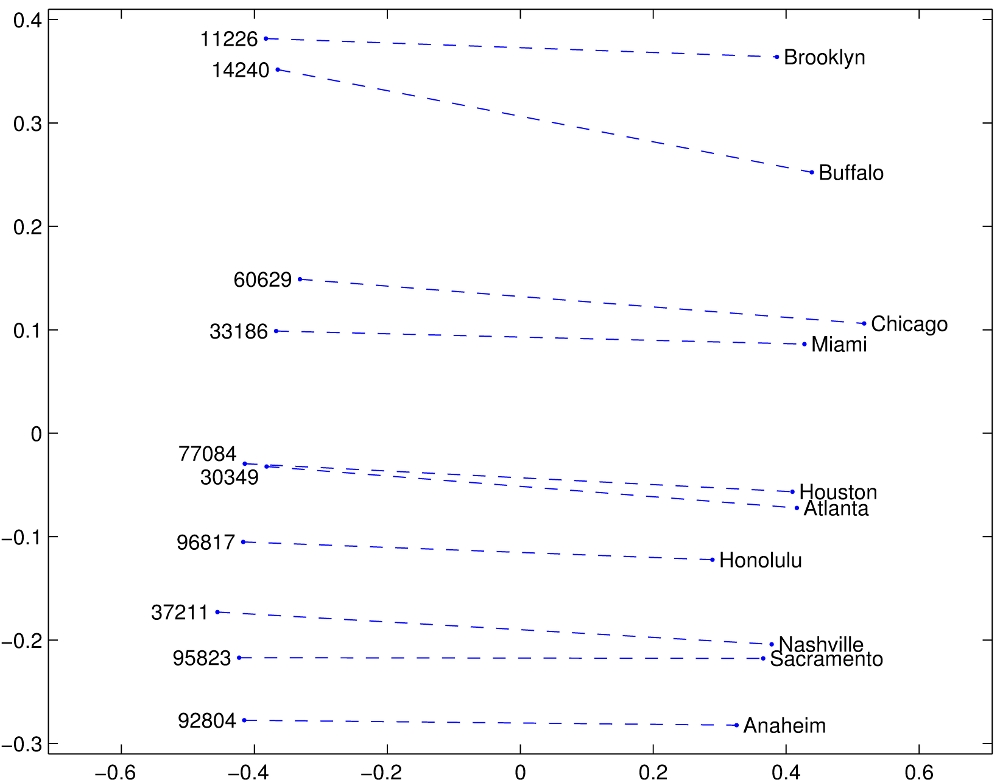
\includegraphics[width=0.45\textwidth]{glove.jpg}
	\centering
	\caption{An example of the linear substructures found in GloVe embeddings (ZIP code - city)}
	\label{fig:gloveExample}
\end{figure} 

Although embeddings exist for over 2 million words (differentiating between upper-case and lower-case letters; useful in the context of may vs. May, for example), the most significant consideration in the embedding step is in dealing with out-of-vocabulary (OOV) tokens. Some works opt to encode OOV tokens as zero or random vectors, believing that meaningful embeddings will be learned through the training process of the entire network. Others use separate character-level embeddings in conjunction with word-level embeddings, while yet others use word-embeddings where each word is treated as a sequence of characters \cite{ELMo}. This point is discussed further in Section \ref{extensions}.

\subsection{Attention Mechanisms}
Sequence-to-sequence (seq2seq; otherwise referred to as encoder-decoder) models are a subset of recurrent neural network models designed to produce variable length outputs from variable length inputs. Originally designed for machine translation \cite{seq2seq} where word \& sentence lengths vary between languages despite sharing the same meaning, these models have proven applicable to a wide variety of NLP tasks, including reading comprehension. To train on input and output sequences of variable length, a seq2seq model uses two recurrent neural networks (each has its own learned weights): the first, the encoder, processes the entire input sequence, embedding it into a fixed-dimension vector space through its final hidden state. The second, the decoder, then takes the final state of the encoder as its initial state; generating outputs until a special stop token is generated. 

\begin{figure}[h]
	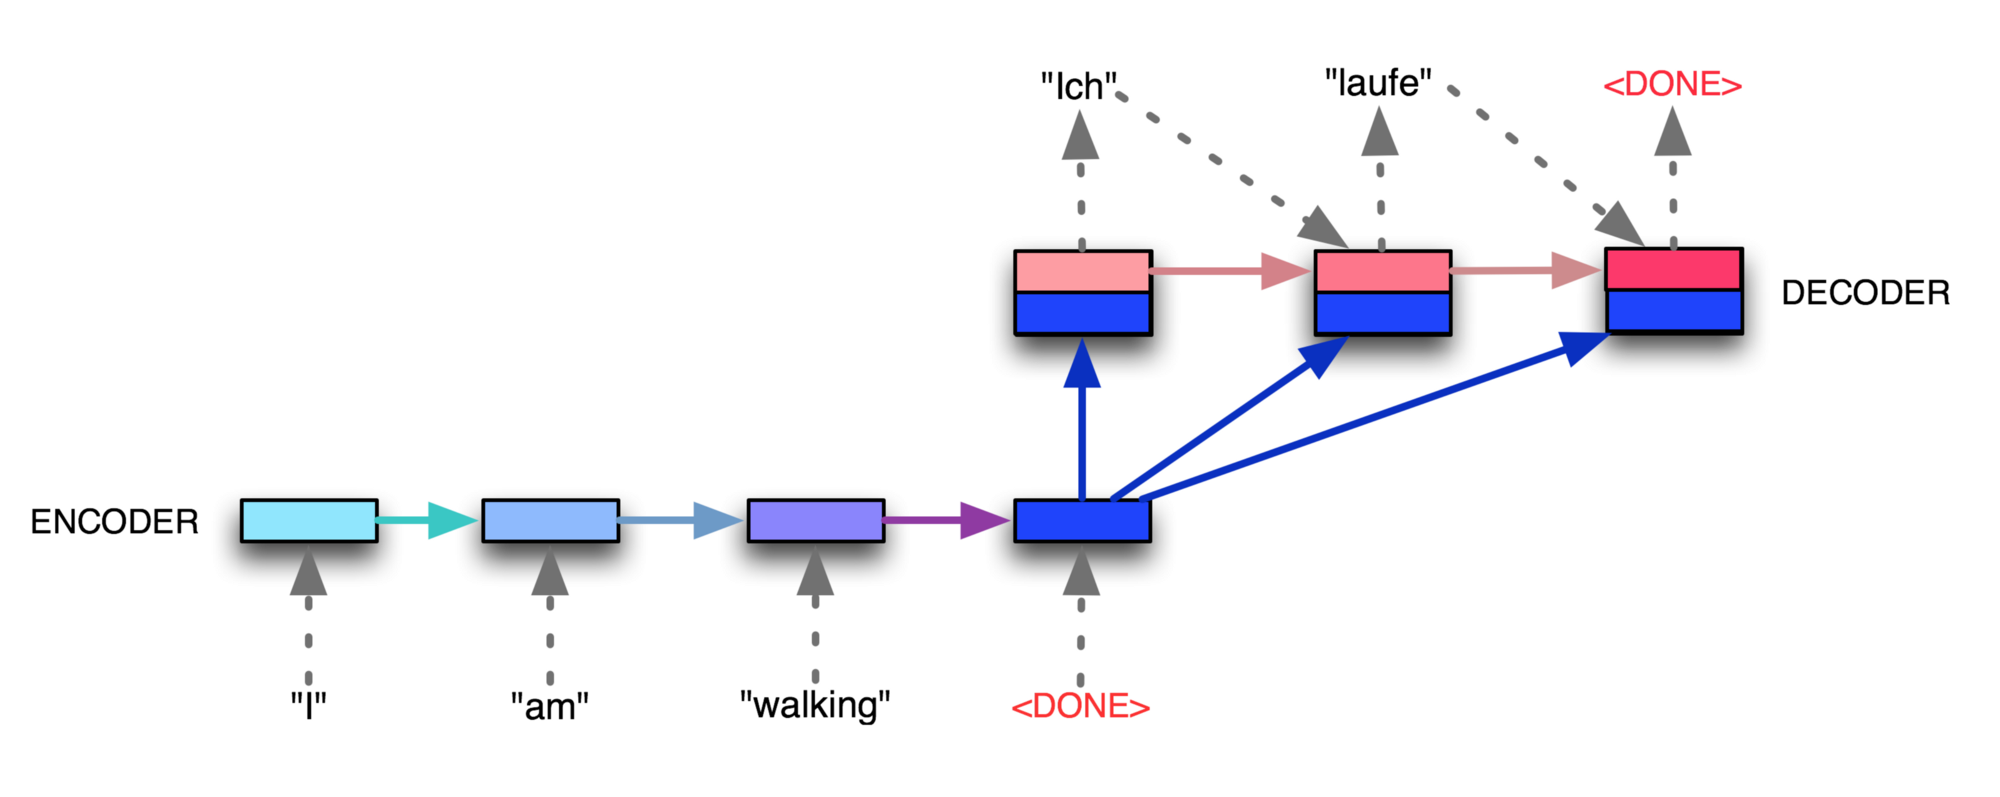
\includegraphics[width=0.6\textwidth]{seq2seq.png}
	\centering
	\caption{Translation (English $\rightarrow$ German) using a seq2seq model}
	\label{fig:seq2seq}
\end{figure}

A major limitation of the original seq2seq model is that the entire input sequence would have to be summarized into one fixed-length vector (referred to as the ``thought vector''), regardless of the length of the input sequence. The thought vector is then the only aspect of the input sequence that the decoder has access to, causing the model to struggle to learn relationships between longer sequences. Attention mechansims combat this by allowing the decoder to ``attend'' to different subportions of the input sequence at every time step of the decoder, allowing both networks to focus on much more localized translations at any one step. Specifically, Bahdanau attention \cite{Bahdanau} works as follows: given an input sequence $x_1, \ldots x_n$, with corresponding encoder outputs $h_1, \ldots h_n$, the output at time $t$ is given by $y_t = \textnormal{RNN}(y_{t-1}, \sum_{i=1}^n w_i^{(t)} h_i)$, where $\sum_{i=1}^n w_i^{(t)} = 1$ for every $t$, giving a natural interpretation as a probabilistic attention over the input sequence. These attention weights also give valuable insights into the reasoning process of the model, as the attention weights produce an interpretable (input length) $\times$ (output length) matrix, as shown in Figure ~\ref{fig:attention}(b). Using additive weights \cite{Luong} has been empirically observed to speed up training, while it has also been suggested that attention weights should not be normalized to the same value at every time step to account for the relative importance of certain subsections \cite{Nallapati}. 

\begin{figure}[h]
	\centering
	\subfloat[Attention mechanism]{{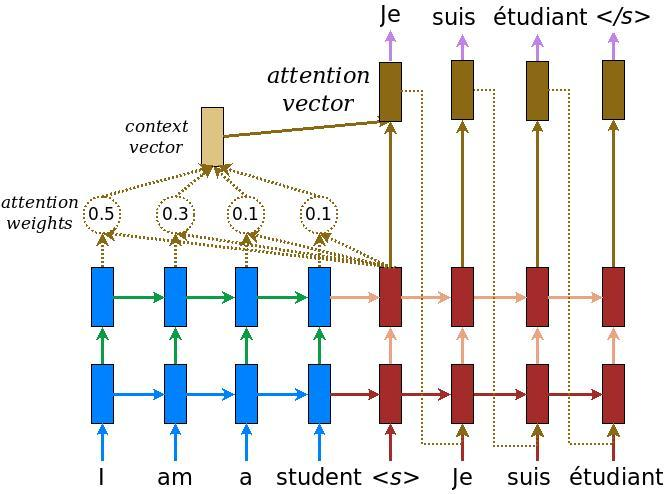
\includegraphics[width=0.35\textwidth]{attention_mechanism.jpg}}}
	\qquad
	\subfloat[Attention weights]{{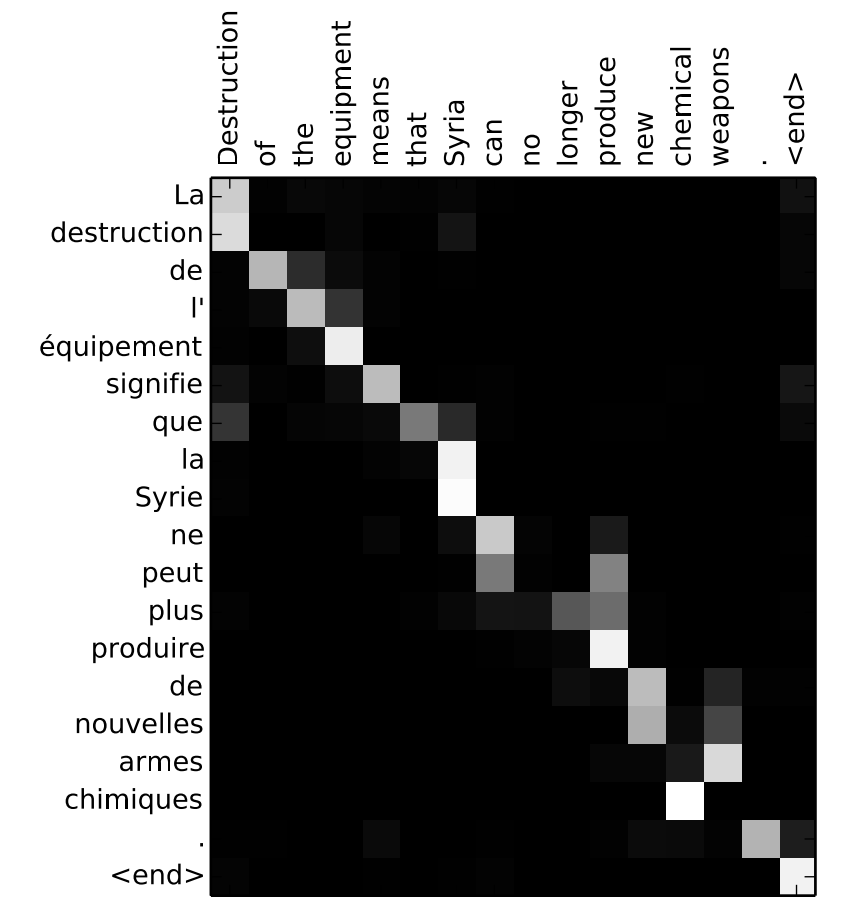
\includegraphics[width=0.35\textwidth]{attention_weights.png}}}
	\caption{Translation (English $\rightarrow$ French) using a seq2seq model with attention}
	\label{fig:attention}
\end{figure}

In the context of reading comprehension, we use attention-based recurrent neural networks to create encodings of one passage of text that are ``aware'' of another passage. This applies most commonly to generating question-aware paragraph encodings so that our algorithm knows where to ``look'' for the answer, but also applies in other settings as discussed in Sections \ref{related} \& \ref{model}.

\subsection{Pointer Networks}
A challenge specific to the SQuAD dataset is that the outputs are categorical labels, where the number of classes varies per sample (it is equal to the number of words in the input sequence). Pointer networks \cite{Ptr-Net} were designed specifically for classification problems whose number of classes is equal to the dimension of the input, such that the network can output ``pointers'' to the input. Originally used to learn planar convex hulls and solutions to the Traveling Salesman Problem, pointer networks are a simplification of a seq2seq model with attention: the attention weights are used as probabilistic pointers. The element of the input ``pointed'' to with the highest probability then becomes the next input to the decoder. 

%% RELATED WORK
\section{Related Work} \label{related}
We present a summary of the three highest scoring single-model (as opposed to ensemble) models on the SQuAD leaderboard as of Feburary 2018, for which there exists a publicly available paper. 

\paragraph{R-Net} (5th as of \today) \\
The R-Net \cite{RNet} model closely follows the structure outlined in Section \ref{background}. The model starts out with two parallel pipelines: one for the paragraph, and one for the question. Each is embedded into a word-level and character-level vector space which are concatenated together, producing a 600-dimensional vector for each word in the paragraph and the question. Each then passes through a bi-directional gated recurrent unit (GRU) \cite{GRU} to learn a higher-level abstraction, before a seq2seq model attends over the question while decoding the paragraph to produce a question-aware paragraph representation. A second seq2seq model is run over this representation attending over itself, before feeding into a pointer network that produces answers. The key contributions of this paper are the self-attention layer, which acts as a ``proofreading'' mechanism for learning long-term dependencies, and a gated attention mechanism that increases model flexibility. 
 
\paragraph{Reinforced Mnemonic Reader} (6th as of \today) \\
The reinforced mnemonic reader model \cite{Mnemonic} starts with similar pipelines (one each for the question and paragraph). First, each word in both the question and paragraph is converted to a vector with GloVe and ELMo \cite{ELMo}. A character level embedding using a bi-directional long short-term memory network (BiLSTM), part-of-speech tags, and and exact match embeddings are also generated for the question and the paragraph. An iterative aligner then aligns the paragraph against the question and against itself. Finally, a variant of a pointer network is used as the answer pointer to make predictions. This variant uses reinforcement learning with the task reward being the difference between the predicted answer and the ground truth. The main contributions of this paper are the use of the reinforcement learning variation of the pointer net and a reattention mechanism that temporarily memorizes past attentions to refine current attentions.

\paragraph{BiDAF} (21st as of \today) \\
BiDAF (bi-directional attention flow) \cite{BiDAF} proposed by the Allen Institute of AI also follows a similar pipeline. Word-level (using GloVe) and character-level (using a CNN \cite{Kim}) embeddings are generated to form vector-space embeddings for all words, with the character-level embeddings proving particularly informative for OOV tokens. Independent representations of the paragraph and question are each passed through bi-directional LSTMs, before feeding into a seq2seq model with attention. The contribution of this paper is in the use of bi-directional attention, i.e. both from paragraph to question and question to paragraph, where the two are combined to produce the final output of the attention flow layer. These pairwise-aware representations are fed through another bi-directional LSTM, before independent fully connected layers are used to generate the pointers. \\ 

Our work this semester has focused on reproducing R-Net, as we felt that their paper was the most detailed, and there exist publicly available implementations in TensorFlow. In hindsight, this determination was not accurate: the paper contains ambiguous phrasing and inconsistent notation throughout (so much so that an entire \href{https://yerevann.github.io/2017/08/25/challenges-of-reproducing-r-net-neural-network-using-keras/}{blogpost} has been dedicated to it), and there are a variety of public implementations because most have struggled to reproduce the results claimed in the paper. However, we take encouragement from the similarity between many of the state-of-the-art models, and hope that the process of deciphering the ambiguity has provided us with a broad understanding of the field of QA systems.

%% MODELS & EXPERIMENTS
\section{Models \& Experiments} \label{model}

\subsection{Fixed Question with Synthetic Data}
Our preliminary experiments focused on smaller models and synthetic, simple tasks. The purpose of this task was simply to test the functionality of the last layer, the pointer network. We generated a synthetic dataset of passages consisting of random sentences describing two fictional people ``he'' and ``she'' going various places, where the task is to learn where ``she'' is at the end of the passage. Since the question is always the same, this is not a full QA task as it is not necessary to feed the question into the model. Paragraphs and sentences were randomized with various locations, prepositions, and adverbs, as illustrated in Figure~\ref{fig:fakeData1}(a). The decision rule that the model would need to learn is exceedingly simple: find the last sentence with ``she'' as the subject, and find the location associated with that sentence.

\begin{figure}[h]
	\centering
	\subfloat[Data generation]{{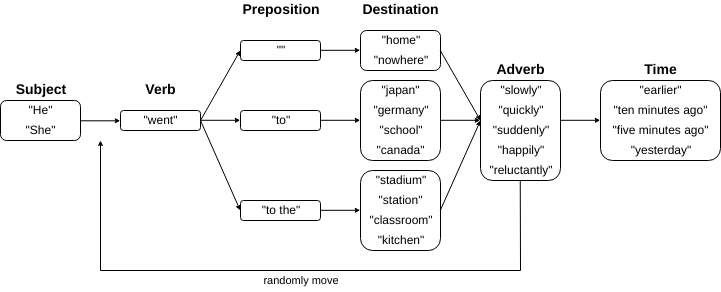
\includegraphics[width=0.5\textwidth]{fake_data1.png}}}
	\qquad
	\subfloat[Model architecture]{{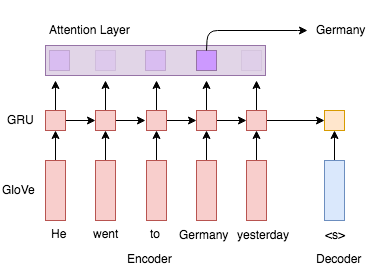
\includegraphics[width=0.3\textwidth]{pointer_net.png}}}
	\caption{Synthetic task 1}
	\label{fig:fakeData1}
\end{figure}

We used a pointer network with a 3 layer (uni-directional) GRU with 50 units in each cell for both the encoder and decoder, with Bahdanau attention. We used 50-dimensional GloVe embeddings, and trained with a learning rate of 0.001 using the Adam optimizer \cite{Adam}. Due to the exceeding simplicity of the task, the model was able to achieve 100\% testing accuracy within 2 epochs. In addition, the pointer probabilities were all approximately equal to 1, leaving little room for analysis and interpretation. This experiment was conducted largely for the purpose of verifying the correctness of our TensorFlow implementation, and the expected accuracy was attained (although faster than expected).  

\subsection{Variable Question with Synthetic Data}
Our second experiment increased the complexity of the task by increasing the number of subjects from 2 to 5, and more significantly, randomizing the question to ask ``Where is \textless subject\textgreater?''. The inspiration behind this dataset is the bAbI \cite{bAbI} project at Facebook AI Research, a project for automatic text understanding and reasoning, that uses children's books as part of their data. \\

\begin{figure}[h]
	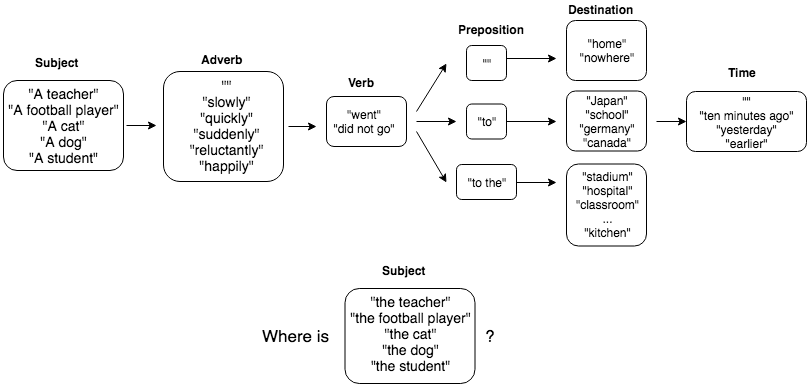
\includegraphics[width=0.5\textwidth]{fake_data2.png}
	\centering
	\caption{Data generation for synthetic task 2}
	\label{fig:fakeData2}
\end{figure}

Unlike for the QA task with a fixed question, this model is required to comprehend the paragraph in the context of the given question. Successful implementations for similar QA tasks modify their representation of the paragraph based on what the question is, and efficiently focus on the most informative regions within the paragraph. This modification is accomplished by the use of attention mechanisms that generate alignments between paragraphs and questions. Inspired by previous implementations \cite{BiDAF}, our model consists of 3 different levels of attention alignment modules which are fed to a pointer net. This structure allows the model to learn from both word-level information as well as higher-level information given the context of entire passages. \\

We generate two levels of abstraction for the question: a higher-level embedding from a RNN, and word-level self-matching. The RNN-embedding updates the word vectors under sequential context, and the word-level self-matching attends over the input to filter the most informative regions. We interpret this layer as a learnable pre-processing layer, which filters irrelevant information prior to any successive computations. This method is inspired by \cite{FusionNet}, which defines multiple levels of abstraction for input words. Our 3 attention alignments are as follows:

\begin{enumerate}
	\item \textbf{Q2P alignment} \\
	Q2P (question-to-passage) alignment aligns the passage with the word-level self-matched question. We hypothesize that this layer learns fairly low-level relationships between the passage and the question.
	
	\item \textbf{High-Q2P alignment} \\
	High-Q2P alignment is an alignment between the RNN-embedded paragraph and the RNN-embedded question. We hypothesize that this layer learns more abstract relationships between the passage and the question.
	
	\item \textbf{P2P alignment} \\
	P2P alignment is a self-matching alignment over the RNN-embedding of the paragraph. This process was first proposed in \cite{RNet} in an attempt to efficiently extract information from long passages where important word-level context may exist sparsely. We hypothesize that this layer learns to attend over informative regions of the paragraph. 
\end{enumerate}
 
\begin{figure}[h]
	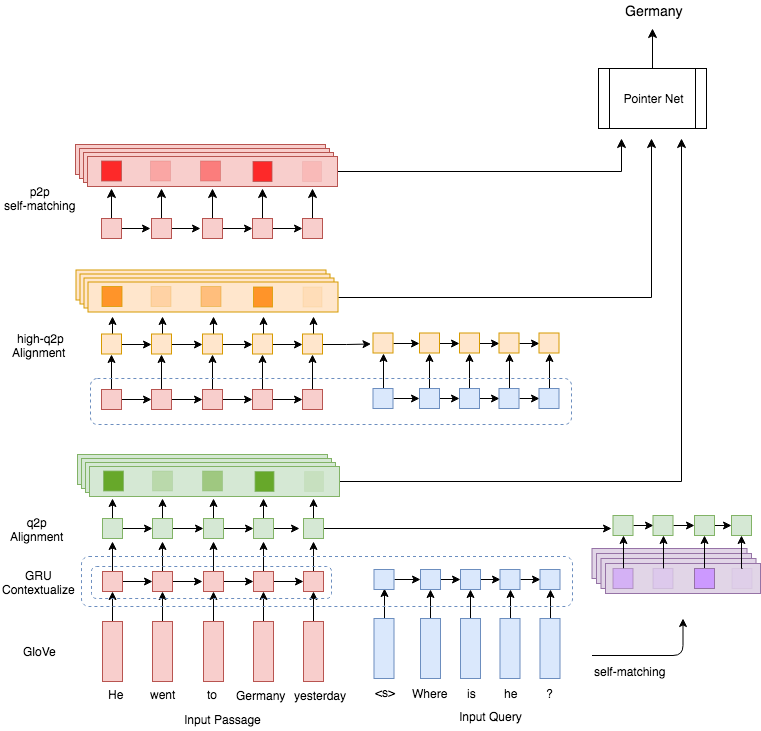
\includegraphics[width=0.65\textwidth]{model.png}
	\centering
	\caption{Model architecture for synthetic task 2}
	\label{fig:QA_model}
\end{figure}

Our interpretations of the role of each alignment are discussed further in Section \ref{discussion}. \\

The 3 attention alignments are concatenated and fed to the final layer, a pointer net, which outputs the exact location of the answer within the input paragraph. We used one-layer bidirectional GRU with 100 units in each cell with 30\% dropout rate for all encoders and decoders in this architecture. We used a slightly higher learning rate of 0.015, which expedites the learning process in order to combat vanishing gradient effects. We used Luong attention \cite{Luong} for all attention layers, which is known to contain less training parameters. In training this model, we observed a severe case of the vanishing gradient problem where the gradient for each neuron is quickly saturated after a few epochs. We were able to mitigate this effect by using Exponential Linear Units (ELU) \cite{ELU} as activation function, and our model converged to 100\% testing accuracy after 30 epochs.

\begin{figure}[h]
	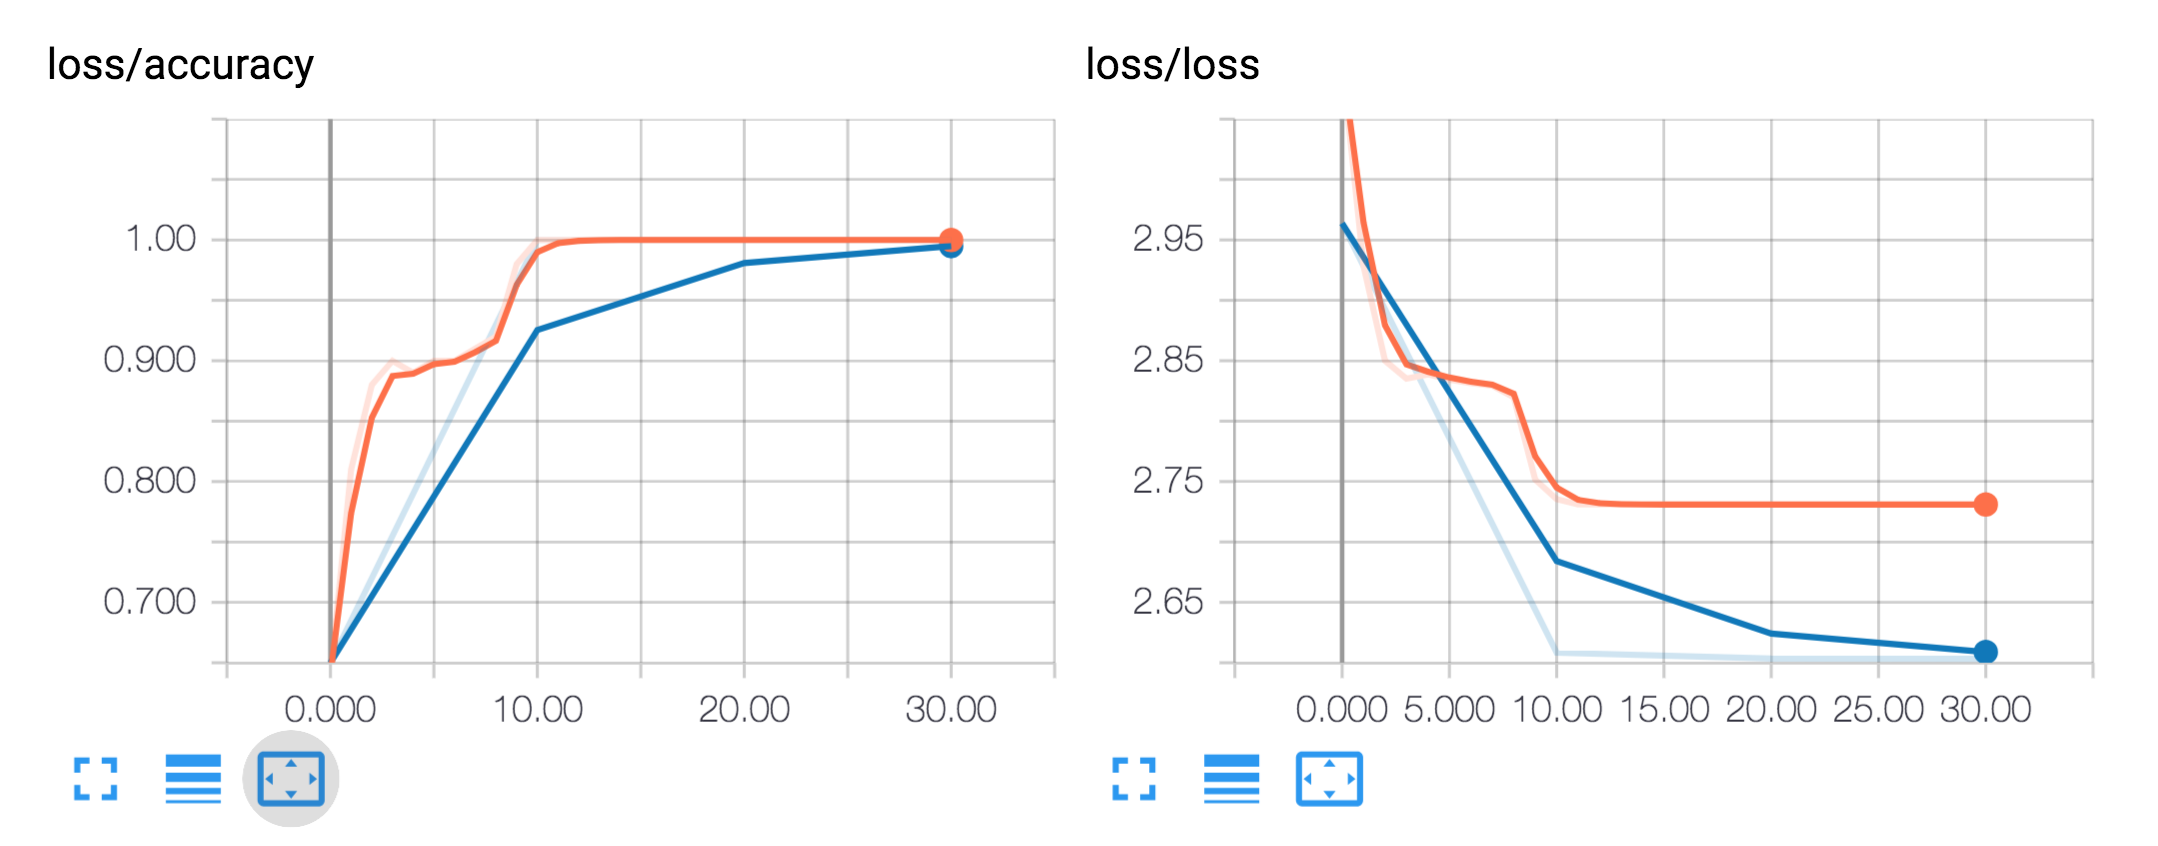
\includegraphics[width=0.65\textwidth]{training.png}
	\centering
	\caption{Training (orange) \& validation (blue) loss (left) \& accuracy (right)}
\end{figure}

%% DISCUSSION
\section{Discussion} \label{discussion}

\subsection{Results}
Attention mechanisms allow us to conceptually hypothesize the ``thought process'' of trained deep learning models, by inspecting the outputs from each attention alignment layer and constructing a heat map of attention weights between two inputs at test time. In this section, we qualitatively interpret attention weights and their functionalities. (See Figures~\ref{fig:heatMaps1} \&~\ref{fig:heatMaps2})

\begin{figure}[h]
	\centering
	\subfloat[Q2P attention weights]{{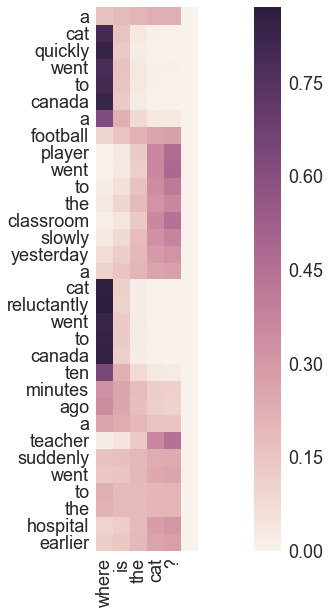
\includegraphics[width=0.27\textwidth]{q2p_heatmap.png}}}
	\qquad
	\subfloat[High-Q2P attention weights]{{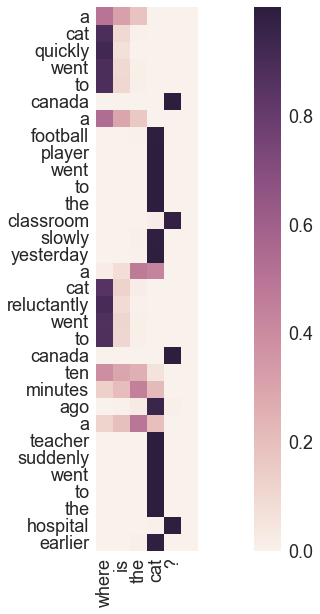
\includegraphics[width=0.27\textwidth]{hq2p_heatmap.png}}}
	\caption{Alignment attention weights}
	\label{fig:heatMaps1}
\end{figure}

\begin{enumerate}[label=(\alph*)]
	\item \textbf{Q2P Alignment} \\
	As hypothesized earlier, Q2P alignment operates on low-level semantics, meaning the model attends based on word-level similarity without any contextual understanding of the passage. The most salient pattern we observe in the figure is the attention weights that scan around the word ``cat'', which corresponds to the subject of the question, ``where is the cat ?'. We can speculate that the model successfully learned to pre-attentively filter out sentences whose subject corresponds with that of the question. Conversely, when the model reads the word ``cat'' in the question, it attends over other subjects of the passage, namely ``football player'' and ``teacher''. We hypothesize that the Q2P alignment layer works as a coarse filter which learns to focus on sentences based on a subject. We speculate the filter is coarse since the attended weight values are fairly low and the resulted heat map is blurred around relevant information. 
	
	\item \textbf{High-Q2P alignment} \\
	High-Q2P alignment synthesizes information from the RNN-embedding of the input sentences, which reflects more abstract contexts of words. Similar to Q2P alignment, High-Q2P alignment also attends over the word ``cat'' while reading the question. We can also observe how refined the filter is compared to the Q2P alignment as it distributes higher attention weights over words. By the end of the question, High-Q2P alignment outputs the heaviest attention weights over 4 candidate answers to the question: ``canada'' (twice), ``classroom'', and ``hospital''. We hypothesize that High-Q2P alignment operates as a more refined filter of words and successfully learns to detect location words, which is the appropriate answer to the question, ``where is \textless subject\textgreater ?''
\end{enumerate}

Although attention layers between different inputs, Q2P alignment and High-Q2P alignment, demonstrate highly intuitive results, the interpretation of self-matching layers are rather challenging. For example, P2P alignment did not seem to learn anything meaningful from our dataset. This is expected behavior since self-matching layers are designed to extract information that sparsely exist in a large corpus of text while our dataset only contains samples of at most 5 short sentences, and therefore the model does not need to utilize the self-matching process. Input self-matching attends strongly over the words ``the cat?'' which is the differentiating factor between all questions within the domain of our synthetic dataset. Given this behavior, we expect that this layer will learn to attend over different information as we increase the variance of question types in the dataset. 

\begin{figure}[!h]
	\centering
	\subfloat[P2P attention weights]{{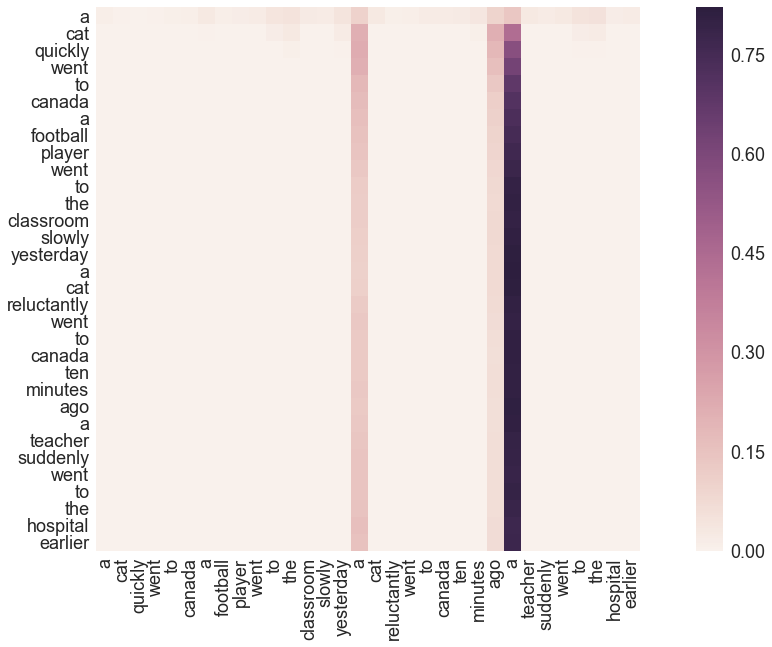
\includegraphics[width=0.47\textwidth]{pp_heatmap.png}}}
	\qquad
	\subfloat[Q2Q attention weights]{{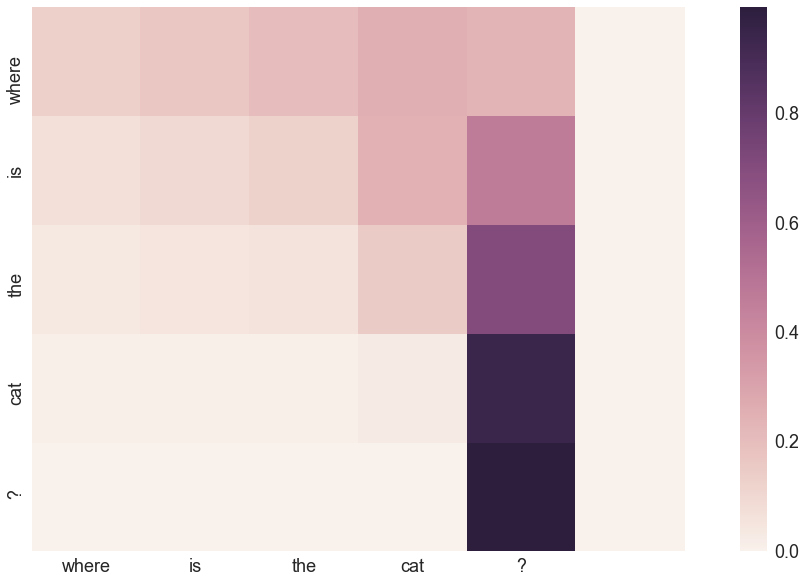
\includegraphics[width=0.47\textwidth]{qq_heatmap.png}}}
	\caption{Self-alignment attention weights}
	\label{fig:heatMaps2}
\end{figure}

\subsection{Implementation Details}
This section is dedicated to implementation difficulties we have experienced to date, as well as workarounds we have been using. As such, this section is more for documenting our procedures than anything else. 

\paragraph{Training Helpers}
\texttt{tf.contrib.seq2seq} ``Helpers'' provide mechanisms to feed in appropriate inputs to the decoder of a seq2seq model. The two that we used in our models are the \texttt{TrainingHelper} and the \texttt{GreedyEmbeddingHelper}. The \texttt{TrainingHelper} passes the ground truth input to the decoder at every time step, regardless of the output at the previous time step (at inference, the input at time $t$ is the output at time $t-1$, or in the case of a pointer network, the element of the input sequence indexed by the output at time $t-1$). Care must be taken to ensure that at inference time, the TensorFlow graph has no dependencies on the \texttt{TrainingHelper}, or the model will have learned nothing useful. On the other hand, the \texttt{GreedyEmbeddingHelper} mimics the procedure at inference time by passing the row of an embedding matrix indexed by the output at the previous time step. A limitation of this mechanism, however, is that the input to the encoder may not be the output of an embedding layer, meaning that we cannot use a fixed embedding matrix. Indexing into the input embedding layer causes us to lose information gained by previous layers, while creating a custom Helper was beyond the scope of our work this semester. The choice between the two is a design decision: feeding in ground truth input at every time step speeds up training, but the greedy helper mimics the auto-regressive nature required at inference. 

\paragraph{Setting Initial States}
We made the decision to set the initial state to be the zero vector for every decoder in our models. Although in a traditional seq2seq model it is common to use the final hidden state of the encoder as the initial state of the decoder, with attention-based RNNs the decoder has access to multiple representations of the input sequence, making this approach no longer suitable in our opinion. The final hidden state of the encoder is likely to depend strongly on the latter portion of the input sequence, but the first step of the decoder is likely to attend over the beginning of the input sequence. Even in the case where this correlation does not hold, we believe that the typical length of a context paragraph makes it unlikely that a fixed-dimension vector is able to capture much about the paragraph beyond a broad summary of the topic. We hypothesize that the initial state is unlikely to make a significant difference to our results, but given that the decoder decodes for a very limited number (equal to the number of pointers, 2) timesteps, this is worth verification next semester.

\paragraph{Training Time}
A significant bottleneck on our work this semester has been the time required to train a complex RNN on relatively long passages of text. Initial attempts to train a model for SQuAD on current CDS servers takes $\approx$40s per batch, equating to approximately 7 hours per epoch. While the scheduled setup of a GPU next semester should help to reduce training time, it remains in our interests to explore other methods to speed up our code. We have identified two potential bottlenecks in our code:
\begin{itemize}
	\item While better than using nested for loops that require TensorFlow to constantly switch between its C backend and Python code, the use of a regular Python class to iterate through batches is sub-optimal. It is our understanding that current best practice is to use queues and the \texttt{tf.data.Data} class, and avoid use of the simpler but slower \texttt{feed\_dict()} method. 

	\item We currently use multiple wrappers defined in \texttt{tf.contrib.seq2seq} in our attention-based RNNs. We believe that the use of a \texttt{tf.while} loop within the \texttt{tf.contrib.seq2seq.dynamic\_decode()} and \texttt{tf.nn.dynamic\_rnn()} methods are largely responsible for our slow training time. Working with lower-level TensorFlow operations and batching similar length inputs together are possible solutions to this problem. Another approach would be to use a different deep learning platform entirely, namely PyTorch, which constructs dynamic computational graphs and is popular for NLP tasks.  
\end{itemize}


%% EXTENSIONS
\section{Extensions} \label{extensions}
\subsection{Feature Engineering}
As evidenced in Section \ref{related}, many recent models follow a similar structure, with minor tweaks focused on improving training time or learning specific (usually long-term) dependencies within the context paragraph. Especially as the state-of-the-art models approach human-level accuracy (as of \today, the top 6 submissions surpass human performance on exact matching answers, although F1 score still trails), it is understandable that recent work has focused on the incremental gains made by these adjustments. 

\begin{figure}[h]
	\centering
	\subfloat[Predicted Answer]{{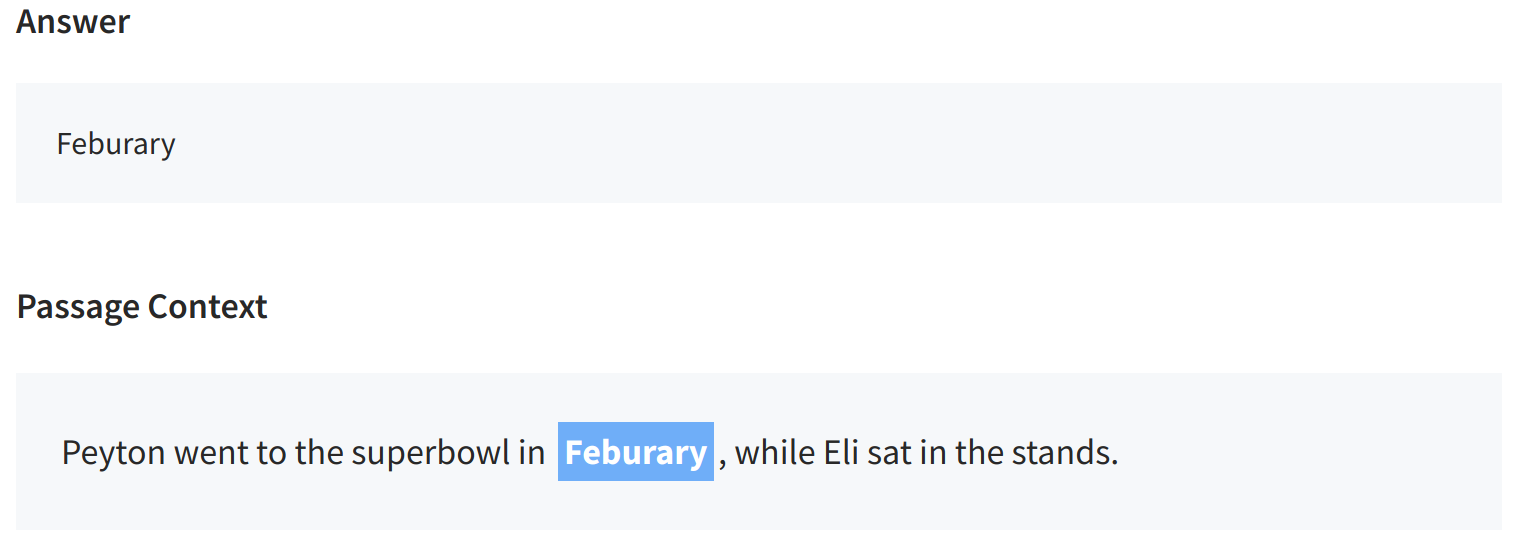
\includegraphics[width=0.45\textwidth]{allen_demo2.png}}}
	\qquad
	\subfloat[Attention weights]{{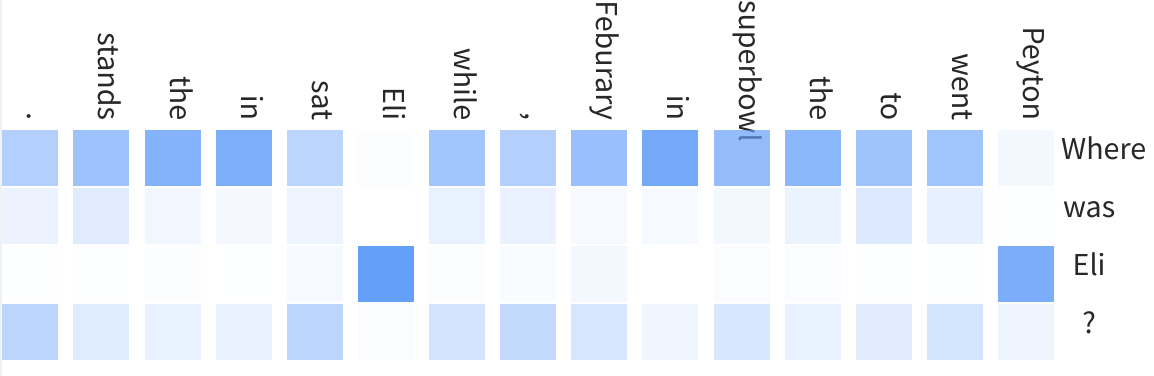
\includegraphics[width=0.5\textwidth]{allen_demo.png}}}
	\caption[caption]{Example output of pre-trained BiDAF model\footnotemark}
	\label{fig:allenDemo}
\end{figure}
\footnotetext{Sample is a reference to Eli \& Peyton Manning: \url{https://www.youtube.com/watch?v=GcnFa7XrKiM}}

However, as illustrated in Figure~\ref{fig:allenDemo}, even state-of-the-art models leave much to be desired in terms of common sense, and interestingly, we find that the BiDAF model struggles to answer questions that our basic model is capable of. The problem with the predicted answer given by BiDAF is two-fold: the first is that ``February'' forms part of the clause associated with ``Peyton'', whereas the question asks about ``Eli''; the second is that ``February'' is very rarely the answer to a question posed using ``where''. Adding parts-of-speech tags as an additional input appear to be a natural way to tackle the second issue, as some models have already. A natural extension to this procedure is simply to take advantage of as much of the existing work in NLP as possible, through resouces such as spaCy\footnotemark\footnotetext{\url{https://spacy.io/}}, which provides named entity recognition and dependency parsing in addition to PoS tags and tokenization. Dependency trees appear useful in tackling the first problem mentioned above (predicted answer is from the wrong clause), but to our knowledge, there do not exist well-established methods of learning from tree-structured data. The learning process behind the generation of dependency trees is one of several topics that we may choose to explore in depth next semester.

\subsection{OOV Tokens}
Having a robust method of dealing with OOV tokens is particularly important when considering our long-term objective of creating a system to synthesize knowledge from textbooks. It is often the OOV words that are the target of questions, and it is important to be able to distinguish between precise definitions of words that may appear similar.

\subsubsection{Character-level Word Embeddings}
Many models, including R-Net, use character-level embeddings to provide information on OOV words. However, ambiguous notation in the paper has caused confusion in public implementations, as the character-tokenized length of a string is obviously different from the word-tokenized length of the same string, but their exact method for aligning the two is unclear. Below we present our understanding of their character-embedding method:

\begin{figure}[h]
	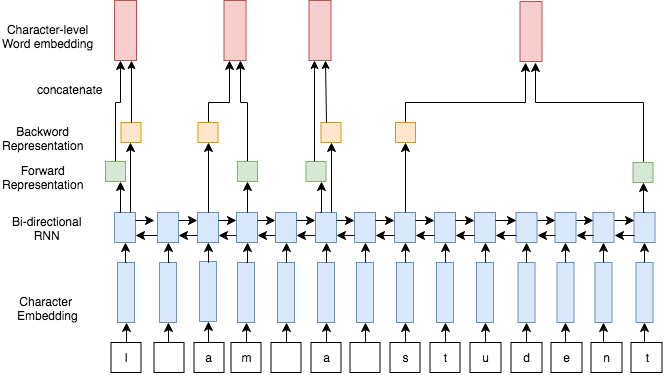
\includegraphics[width=0.55\textwidth]{char_word2vec.png}
	\centering
	\caption{Character-level RNN for encoding OOV tokens}
	\label{fig:charRNN}
\end{figure}

We first generate vector-space embeddings of characters by treating every word as a ``bag-of-characters''. Using pre-trained GloVe vectors, we generate character embeddings by taking a weighted sum of every word in the GloVe vocabulary containing that character, where the weight is equal to the frequency of the character in the word. For example, the character embedding of the character ``a'' is a weighted sum of the word vectors for ``apple'', ``banana'', ``orange'', etc., where the weights are 1, 3, 1 respectively. The words containing regular characters in the alphabet are almost entirely unrelated in terms of meaning, but this method can be useful in providing embeddings for numbers and special characters; it is also important to keep in mind that these simply serve as an alternative to one-hot encodings or random initializations. \\

As shown in Figure~\ref{fig:charRNN}, taking the output at the final character of each word produces vectors that can be concatenated with GloVe embeddings to produce unified embeddings of both passages. We hypothesize that using a LSTM in this setting generates unique embeddings for every word in a manner analogous to a hidden Markov model, and that the forget gate will learn to ``reset'' upon seeing a space.

\subsubsection{R-R-Net}
To generate more context-aware embeddings of OOV tokens, we propose an approach that takes advantage of the fact that we are provided a paragraph of relevant information and a QA system. A passage that contains the name ``Barack Obama'' can be augmented with information that Obama is a former president of the United States by simply using an existing QA model. This helps to contextualize the passage in a manner that could not be achieved by simply registering ``Obama'' as a unique token.

\section{Notes}
All code related to this report can be found at \url{https://github.com/CornellDataScience/QuACC}, \\
\url{https://github.com/yujiakimoto/ptr-net}, and \url{https://github.com/Kenta426/neural-attention} \\
\\
Our submission to BOOM 2018 was the recipient of the Capital One award.

\newpage
\bibliographystyle{apalike}
\bibliography{references}

\end{document}
